%%%%%%%%%%% Exposición 03
\subsection[Expositor: Juan Manuel Díaz Quiñonez.]{Iluminación de polígonos con refelctores.}
\textbf{Obejetivo:} Cotas sobre el número de reflectores suficientes para iluminar un polígono simple.\newline

\textbf{Desarrollo:} Para cada vértice $p_i$ en el polígono se asignan pesos de $\alpha_i$ correspondiente
al ángulo de iluminación a partir de $p_i$. Cabe mencionar que no es cierto que para cada $p_i$ corresponda
un $\alpha_i$ necesariamente.\newline

Dado un subconjunto S de los vértices de P, decimos que $S$ ilumina a P si todo punto de P es visible desde algún
vértice en $S$. Asociaremos un peso a $S$ igual a la suma de los pesos de los elementos de $S$.

\begin{center}
  \textbf{Teo 1.} Todo polígono $P$ con $n$ vértices tiene un subconjunto $S$
  que lo ilumina de tal manera que el peso de $S$ es a lo más
  \[\frac{(n - 2)\pi}{3}.\]
  Para cada $\epsilon > 0$ existen polígonos tales que
  no tienen conjuntos de vértices que los iluminen de peso
  \[\frac{(n - 2)\pi}{3} - \epsilon.\]
\end{center}


\begin{center}
  \textbf{Teo 2.} Para cualquier $\epsilon > 0$, existen polígonos simples que no
  pueden ser iluminados con reflectores de tamaño menor o igual a $\pi - \epsilon$
  aún permitiendo un reflector por vértice. A nosotros nos importará demostrar que esto es cierto
  para $\epsilon \geq \frac{1}{2}$.
\end{center}

\begin{center}
  \textbf{Teo 3.} Todo polígono ortogonal sin agujeros puede iluminarse
  con a lo más
  \[\lfloor \frac{3n - 4}{8} \rfloor\]
  reflectores ortogonales.
  
  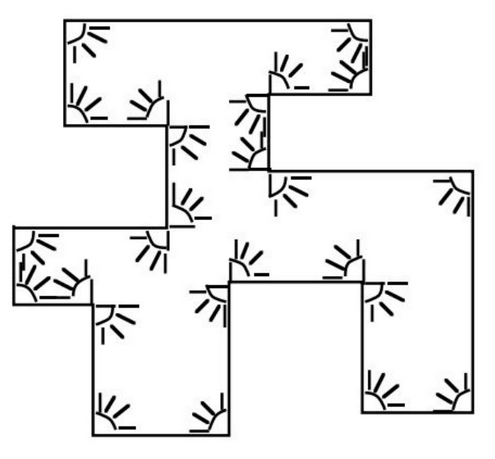
\includegraphics[scale=0.40]{./Im1.png}\\[0.4cm]
\end{center}

\begin{center}
  \textbf{Teo 4.} Todo polígono ortogonal $P$ con $h$ agujeros y $n$ vértices
  puede iluminarse con a lo más
  \[\lfloor\frac{3n + 4(h-1)}{8}\rfloor\]
  reflectores ortogonales colocadas sobre los vértices de $P$.
\end{center}

\begin{center}
  \textbf{Teo 5.} Todo polígono ortogonal $P$ con $n$ vértices puede
  iluminarse con a lo más
  \[\lfloor \frac{n}{4}\rfloor\]
  reflectores sobre la frontera de $P$.
  Dichos reflectores pueden ser localizados
  en tiempo lineal. Resultado mostrado en la exposición de \textit{Ares Castro Romero.}
\end{center}

